\documentclass[herrin-thesis.tex]{subfiles}
\begin{document}

\section{Motivation}
\label{sec:muon:motivation}
One potential source of background in EXO-200 is unstable isotopes of common elements, created by neutron activation. The largest source of these neutrons is spallation by cosmic ray muons. Indeed, EXO-200 is located underground to reduce cosmic activation. The energy loss rate \((d E/d x)\) for relativistic muons has a broad minimum between \SIlist{1;10}{\GeV}, and increases slowly for higher energies. Therefore, some muons produced in the upper atmosphere can still travel deep underground.

Neutrons from these muons can capture on detector materials or the HFE, producing high-energy gamma rays that might Compton scatter in the detector and leave behind energy close to the Q value for \xenon{136}. These gamma rays are prompt, and so can be vetoed if the muon can be tagged. A neutron capture on \xenon{136} produces \xenon{137}, an isotope that beta decays with a Q value of 3.8 MeV, which means the beta particle produced in the decay could have an energy close to the Q value of \xenon{136}. The half life of \xenon{136} is 3.8 minutes, and so vetoing becomes more difficult. But a good measurement of the muon flux can put constraints on the amount of \xenon{137} decays observed.

\section{Identifying Muons}
\label{sec:muon:id}
Muons that reach underground have typical energies of \SIrange{1}{100}{\GeV}, a range in which they are minimally ionizing. Those that pass through the detector typically leave a straight line of ionization along their path. Like any energy deposition in EXO-200, some of the energy deposited becomes scintillation light, while the remaining ionization is drifted and collected. Thus, a muon passing through EXO-200 will show a bright flash of light, followed by ionization across many wire channels, linearly spread in time. \Cref{fig:muon:eventdisplay} shows a typical example. This distinct linear trail provides a means to tag the muon.

\begin{figure}[htbp]
\centering
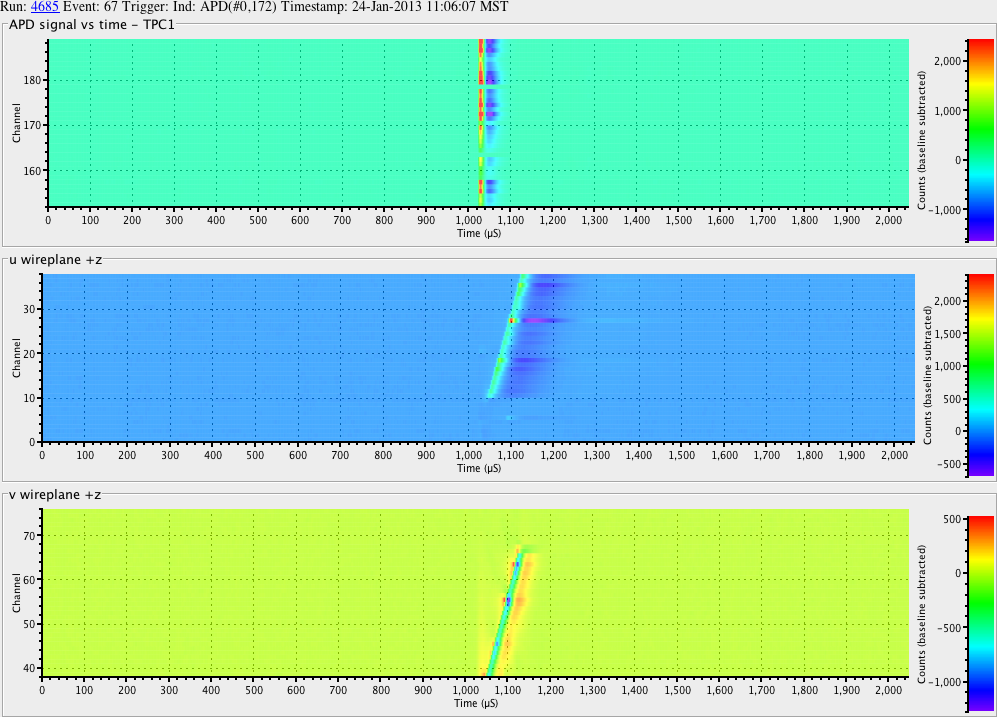
\includegraphics[width=1\columnwidth]{./plots/muon_eventdisplay_run_4685_ev_67.png}
\caption[A muon passing through EXO-200]{The event display for a muon passing through EXO-200. The upper panel shows the APDs versus time, displaying the flash of light when the muon passes through. The middle (lower) panel shows u (v) wire channels versus time, showing the characteristic linear trail of ionization.}
\label{fig:muon:eventdisplay}
\end{figure}

\subsection{Identifying Muons with the Hough Transform}
The Hough transform\cite{Hough:1959fk}\cite{Duda:1972:UHT:361237.361242} is an algorithm originally used to look for tracks in bubble chamber photos. A line can be completely parameterized by the angle \(\eta\) it makes with an axis, and the perpendicular distance \(r\) from the line to the origin. The Hough transform maps a pixel in an image to all possible lines that can pass through that pixel, which looks like a sinusoidal curve in \((\eta, r)\) space. If some of the pixels form a line, then these curves will converge at the point corresponding to that line.

This can be applied to EXO-200 to look for muons. First, ionization deposits are identified by simply looking at the collection wire channel waveforms and looking for the waveform rising a set threshold above its baseline. A ``hot spot'' is associated with the time value at which the waveform peaks above this threshold. The induction wires are analyzed the same way, except looking for the waveform dipping below its baseline. The Hough-transformed hot spots are placed in a histogram, and the bin with the most entries is used to reconstruct the projection of the muon's track onto the wire planes. \Cref{fig:muon:houghtransform} shows an example.

\begin{figure}[htbp]
\centering
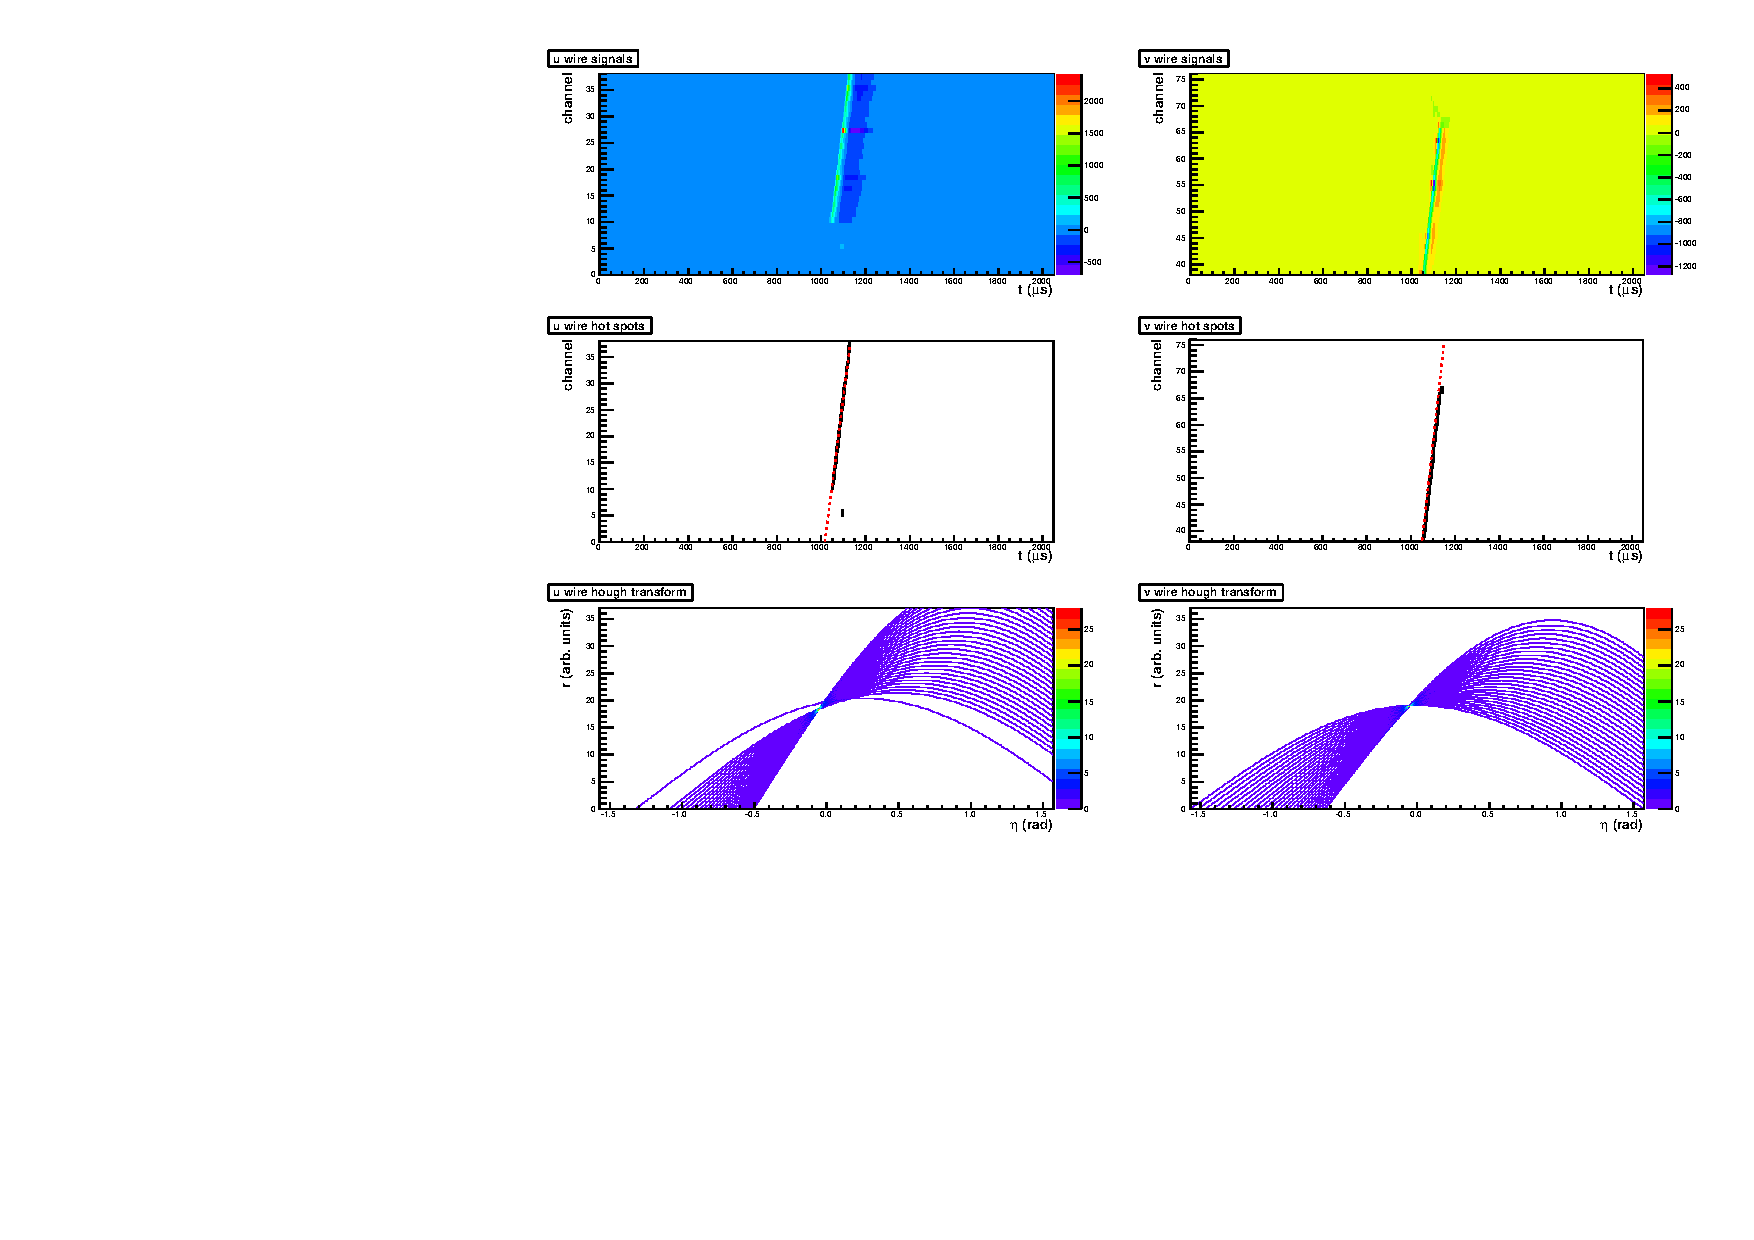
\includegraphics[width=1\columnwidth]{./plots/muon_houghtransform_run_4685_ev_67.pdf}
\caption[Identifying a muon with the Hough transform]{The Hough transform used to identify and reconstruct a muon passing through EXO-200. The left side shows collection wire channels, and the right side shows induction wire channels. The upper panels show the raw waveforms, baseline subtracted. The middle panels shows the identified hot spots in the waveforms in black, and the reconstructed tracks in red. The lower panels show the Hough transforms of the hot spots above, which converge on the point corresponding to the red line above.}
\label{fig:muon:houghtransform}
\end{figure}

After passing a check for noise (described in \Cref{app:noisetagger}) and a check for a large amount of scintillation light, an event will be tagged as a muon if it has good tracks in both the induction and collection wire planes in at least one TPC. A ``good'' track must be reconstructed from at least 5 hot spots that lie along the reconstructed track, or at least 3 hot spots along the track if fewer than 5 total spots were found.

The Hough transform reconstructs the projection of the muon's path onto the wire planes. Since the drift velocity and wire spacings are well known, these projections can be translated back to an incident angle for the muon.

\subsection{Validation with Monte Carlo Simulations}
In order to validate this muon tagging algorithm, 2 million muons were generated in the EXOSim GEANT4 simulation of the EXO-200 detector. The overall efficiency of the tagging depends on the angular distribution of the incident muons (for example, one could imagine a pathological scenario in which all muons were parallel to the wires in one plane). The angular distribution underground is approximated\cite{miyake:1973} by
\begin{equation}
\label{eq:muon_angular_distribution}
\frac{dN}{d\Omega} \propto \left (\cos \theta \right)^{1.53}e^{-8\times10^{-4} h \left(\sec \theta -1\right)}
\end{equation}
where \(\theta\) is the zenith angle and \(h\) is the vertical depth in \si{\hecto\gram\per\square\centi\meter} (\SI{1}{\hecto\gram\per\square\centi\meter} is equivalent shielding to one meter of water). For WIPP, previous experiments have measured \(h\) to be \(1585^{+11}_{-6}\) \si{\hecto\gram\per\square\centi\meter}\cite{Esch:2004zj}. This distribution is a good approximation for \(\theta < \pi/3\).

The energy distribution for muons underground can also be approximated\cite{Gaisser:1990kx}. The distribution for muons at the surface is given by
\begin{equation}
\label{eq:muon_surface_distribution}
\frac{dN}{dE} \propto E^{-2.7}\left(\frac{1}{1+\frac{1.1 E \cos \theta}{115}} + \frac{0.054}{1+\frac{1.1 E \cos \theta}{850}}\right)
\end{equation}
for \(E\) in \si{\GeV}. The flux underground is then
\begin{equation}
\label{eq:muon_underground_distribution}
\frac{dN}{dE} = \frac{dN}{dE_0}e^{b h \sec \theta}
\end{equation}
where \(b E\) defines the rate of continuous energy loss for muons. \(b\) is about \SI{4d-6}{\g\per\square\cm} for standard rock. This makes the substitution
\begin{equation}
\label{eq:muon_E0_def}
E_0 = e^{b h \sec \theta}\left(E + \epsilon\right) - \epsilon
\end{equation}
which is the average energy of surface muons that pass through \(h\sec\theta\) of material and emerge with energy \(E\). The parameter \(\epsilon\) is a critical energy above which discrete energy losses dominate, rather than continuous losses described by \(b\). For standard rock, \(\epsilon\) is about \SI{500}{\GeV}.

Muon events were simulated by first picking an azimuthal angle \(\phi\) uniformly from \(\left(-\pi, \pi\right]\) and a zenith angle \(\theta\) from \cref{eq:muon_angular_distribution}. The energy was selected in a range of \SIrange{1}{1000}{\GeV} from \cref{eq:muon_underground_distribution} for the selected zenith angle. A point was chosen uniform randomly in the cylindrical TPC volume, and a muon was generated \SI{3}{\meter} from this point with the selected energy and incident angles. Positively charged muons were generated in a 1.25 ratio to negatively charged muons. The ``standard rock'' values for \(b\) and \(\epsilon\) were used, and the depth \(h\) was varied 10\% around \SI{1585}{\hecto\gram\per\square\centi\meter} to account for systematic effects of the angular distribution on efficiency.

\subsection{Efficiency}
Overall, of two million simulated events, 864138 were tagged as muons by the algorithm described above. This is an overall efficiency of \(42.3 \pm 0.1\)\%. However, the geometry of the detector means that the efficiency will be a function of the incident muon angle. \Cref{fig:muon_efficiency} shows the efficiency of detecting muons based on the ratio of muons reconstructed in an angular bin to muons simulated in that bin. This is useful for estimating the true flux in a bin. \Cref{fig:muon_correct_ratio} shows the ratio of muons correctly reconstructed to those incorrectly reconstructed in a bin. This is useful for eliminating bins that have a high misreconstructed rate from measurements that require knowledge of incident angles.

 \begin{figure}[htpb]
 \centering
 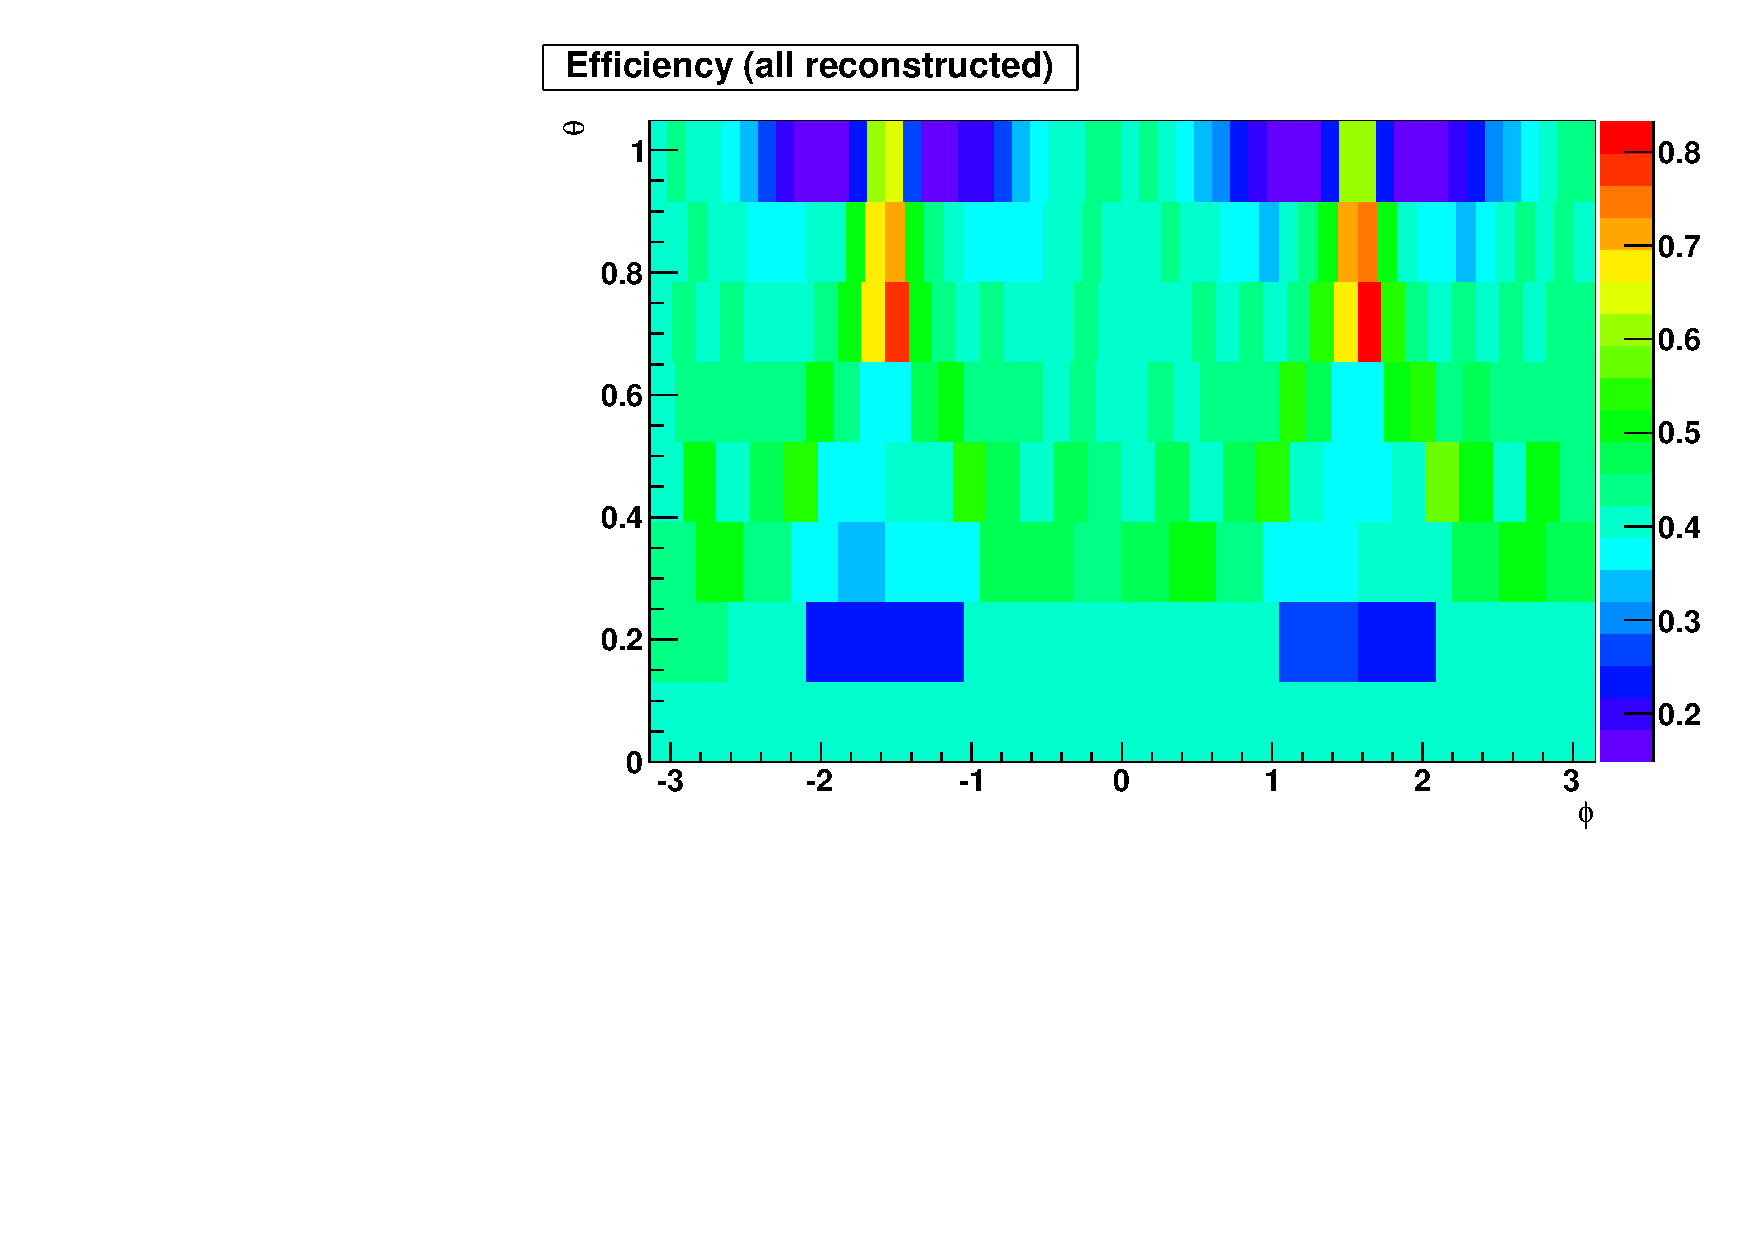
\includegraphics[width=0.8\textwidth]{./plots/muon_efficiency.pdf}
 \caption[Efficiency of reconstructing muons as a function of angle]{The ratio of muons reconstructed in an angular bin to the muons simulated in that bin. This includes muons incorrectly reconstructed, so that this can be used to estimate a total flux. Only \(\theta < \pi/3\) is considered, since the angular distribution used is not good for larger angles.}
 \label{fig:muon_efficiency}
 \end{figure}

 \begin{figure}[htpb]
 \centering
 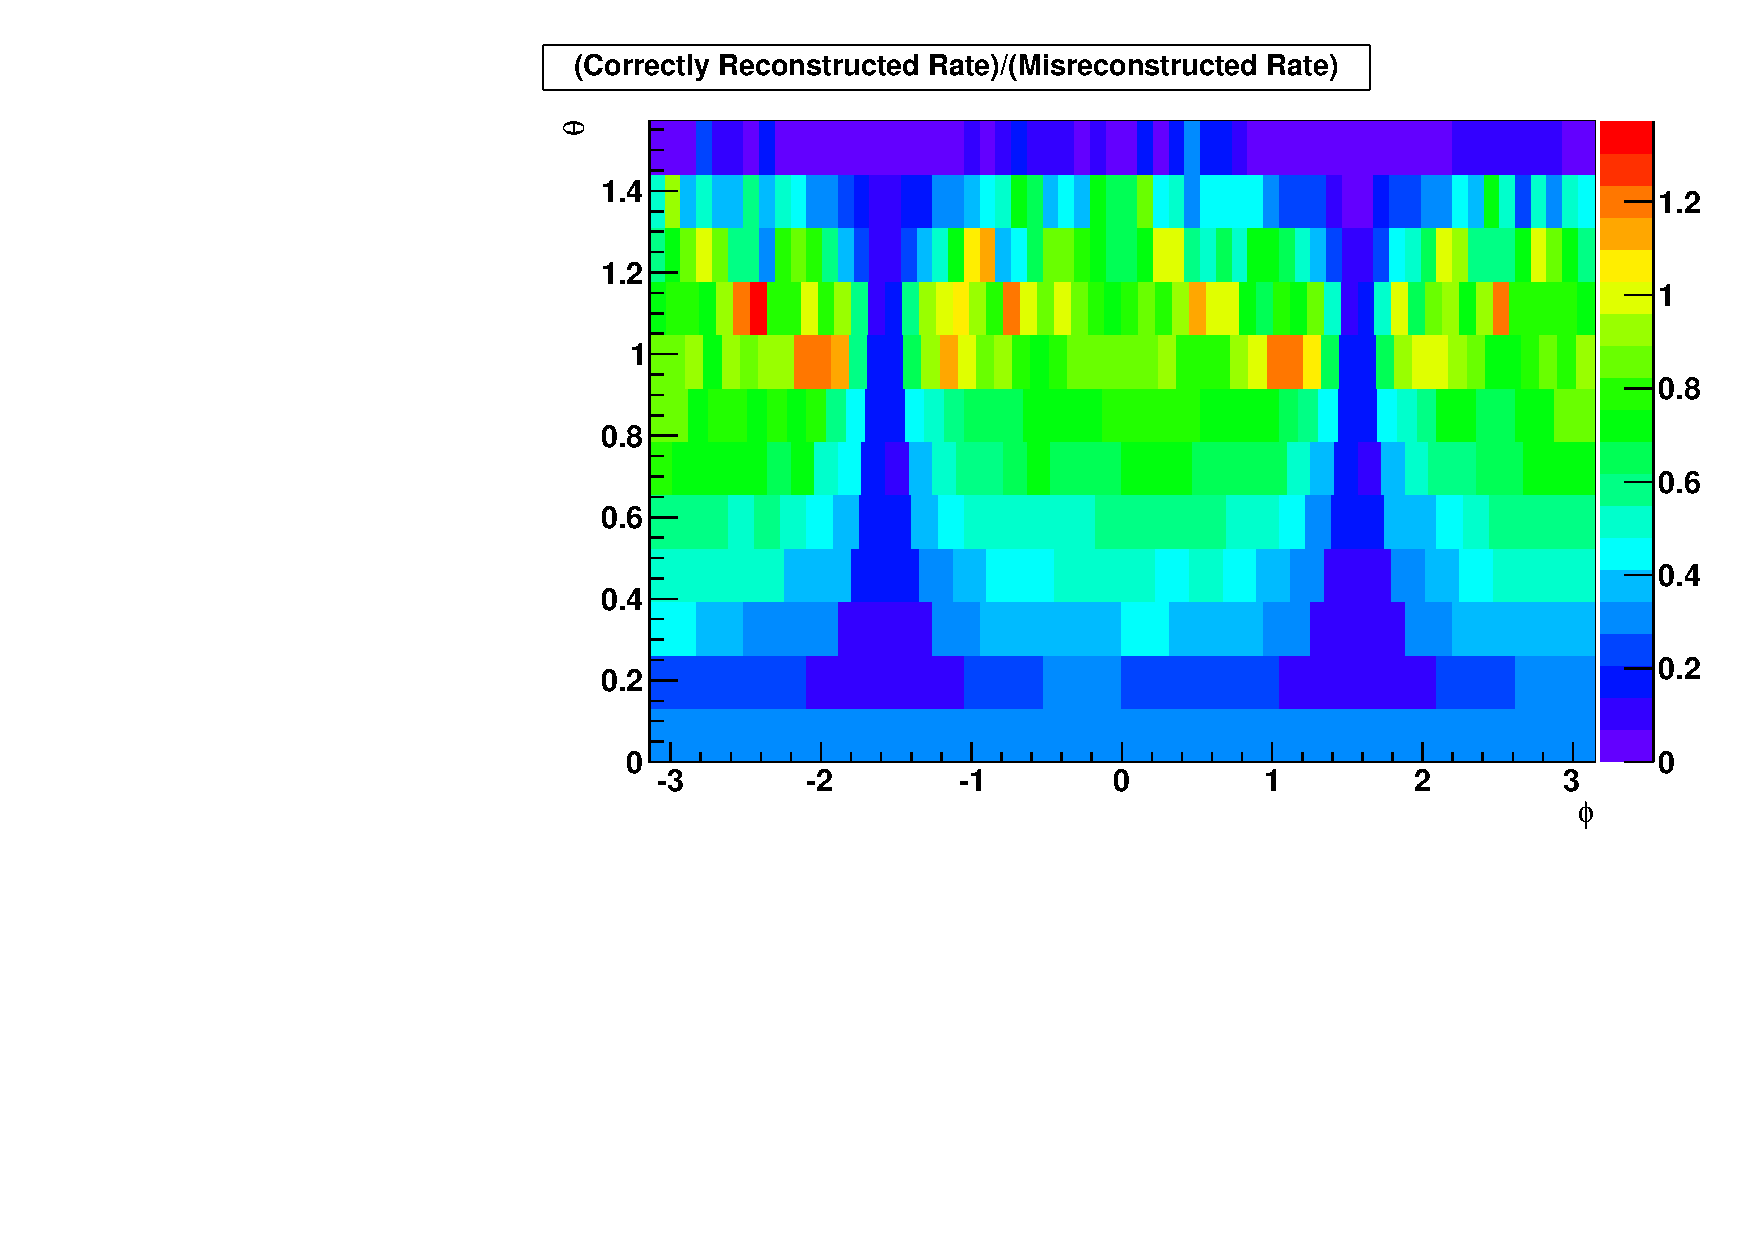
\includegraphics[width=0.8\textwidth]{./plots/muon_correct_ratio.pdf}
 \caption[Ratio of correct to incorrect reconstructions]{The ratio of correctly reconstructed muons to incorrectly reconstructed muons as a function of angle. Note the low correct rate at \(\phi = \pm \pi/2\), which is due to the degeneracy of muons parallel to the wire planes. The azimuthal angle is on the horizontal axis, while the zenith angle is on the vertical axis. The binning attempts to have bins of similar solid angle, save for the zenith bin.}
 \label{fig:muon_correct_ratio}
 \end{figure}

For a particle incident from zenith angle \(\theta\) and azimuthal angle \(\phi\), the effective area of a cylinder on its side is
\begin{equation}
A(\theta,\phi) = \pi r^2 |\cos(\phi)|\sin(\theta) + 2 r h \sqrt{1-\sin(\theta)^2 \cos(\phi)^2}
\end{equation}
when \(\phi=0\) is parallel to the cylinder's axis and where \(r\) is the cylinder's radius and \(h\) is its height.

\end{document} 